\documentclass[14pt]{extarticle}

\usepackage{fontspec}
\setmainfont{Times New Roman}

% размер полей
\usepackage{geometry}
\geometry{a4paper, top=2cm, bottom=2cm, right=1.5cm, left=3cm}

 %debugging
%\usepackage{showframe}

% полуторный интервал
\usepackage{setspace}
\onehalfspacing

% абзацный отступ
\setlength{\parindent}{1.25cm}

% выравнивание текста по ширине
\sloppy

% списки
\usepackage{calc} % арифметические операции с величинами
\usepackage{enumitem}
\setlist{
    nosep,
    leftmargin=0pt,
    itemindent=\parindent + \labelwidth - \labelsep,
}

% подписи к рисункам и таблицам
\usepackage{caption}
\renewcommand{\figurename}{Рисунок}
\renewcommand{\tablename}{Таблица}
\DeclareCaptionFormat{custom}
{
    \textit{#1#2#3}
}
\DeclareCaptionLabelSeparator{custom}{. }
\captionsetup{
    % хз какой это размер - 12 или нет, но выглядит меньше 14
    font=small,
    format=custom,
    labelsep=custom,
}

% картинки
\usepackage{graphicx}

% колонтитулы
\usepackage{fancyhdr}

% картинки и таблицы находятся именно в том месте текста где помещены (атрибут H)
\usepackage{float}

% таблицы
\usepackage{tabularray}

\graphicspath{ {7.2.2/models/} }
\begin{document}
\pagestyle{fancy}
\fancyhead{}
% disable header
\renewcommand{\headrulewidth}{0pt}
\fancyfoot[L]{Дубровских гр 221-361}
\fancyfoot[C]{ЛР 7.2.2}
\fancyfoot[R]{Продажа автотранспорта}
\singlespacing

\newpage
\begin{center}
    Министерство науки и высшего образования Российской Федерации
    Федеральное государственное автономное образовательное учреждение

    высшего образования

    \guillemotleft МОСКОВСКИЙ ПОЛИТЕХНИЧЕСКИЙ УНИВЕРСИТЕТ\guillemotright

    (МОСКОВСКИЙ ПОЛИТЕХ)
\end{center}
\noindent
\bigbreak
\bigbreak
\bigbreak
\bigbreak
\begin{center}
    ЛАБОРАТОРНАЯ РАБОТА 7.2.2

    По курсу Проектирования пользовательских интерфейсов в веб

    \textbf{Изучение критериев и принципов шрифтового оформления контента для веб. Оформление текста в интерфейсе}
    \bigbreak
    \bigbreak
    \bigbreak
    \bigbreak
    ТЕМА

    \guillemotleft\textbf{САЙТ ДЛЯ ПРОДАЖИ И ПОИСКА АВТОМОБИЛЕЙ}\guillemotright
\end{center}
\noindent
\bigbreak
\bigbreak
\bigbreak
\bigbreak
\bigbreak
\bigbreak
\bigbreak
\bigbreak
\bigbreak
\bigbreak
\hfill Выполнил

\hfill Дубровских Никита Евгеньевич

\hfill Группа 221-361
\bigbreak
\bigbreak
\bigbreak
\hfill Проверил

\hfill Натур ВВ
\vfill
\begin{center}
    Москва, 2024
\end{center}
\newpage
\onehalfspacing


\begin{center}
    \textbf{Лабораторная работа 7.2.2}

    \textbf{Изучение критериев и принципов шрифтового оформления контента для веб. Оформление текста в интерфейсе}
\end{center}

\textbf{Цель работы:} оформить текст в интерфейсе в соответствии с принципами подбора типографики, верстки, строения текста и требованиями веб-технологий
\bigskip

\textbf{Задачи:}

\begin{enumerate}
    \item Изучить и зафиксировать в отчете критерии и принципы подбора шрифтов для текстового контента для веб.
    \item Провести анализ (идентификацию) типографики сайтов-аналогов. Сделать вывод
    \item Подобрать типографику (шрифты в кириллице), в том числе шрифтовые пары, для всех текстовых элементов интерфейса проектного сайта
    \item Подобрать для примера типографский контент веб-страниц (заголовки, подзаголовки, несколько предложений основного текста) 
    \item Проверить коэффициент контрастности выбранного шрифта и фона страниц, блоков и элементов сайта.
\end{enumerate}
\bigskip

\begin{itemize}
\end{itemize}
\bigskip

\noindent
\begin{minipage}{\linewidth}
    \fbox{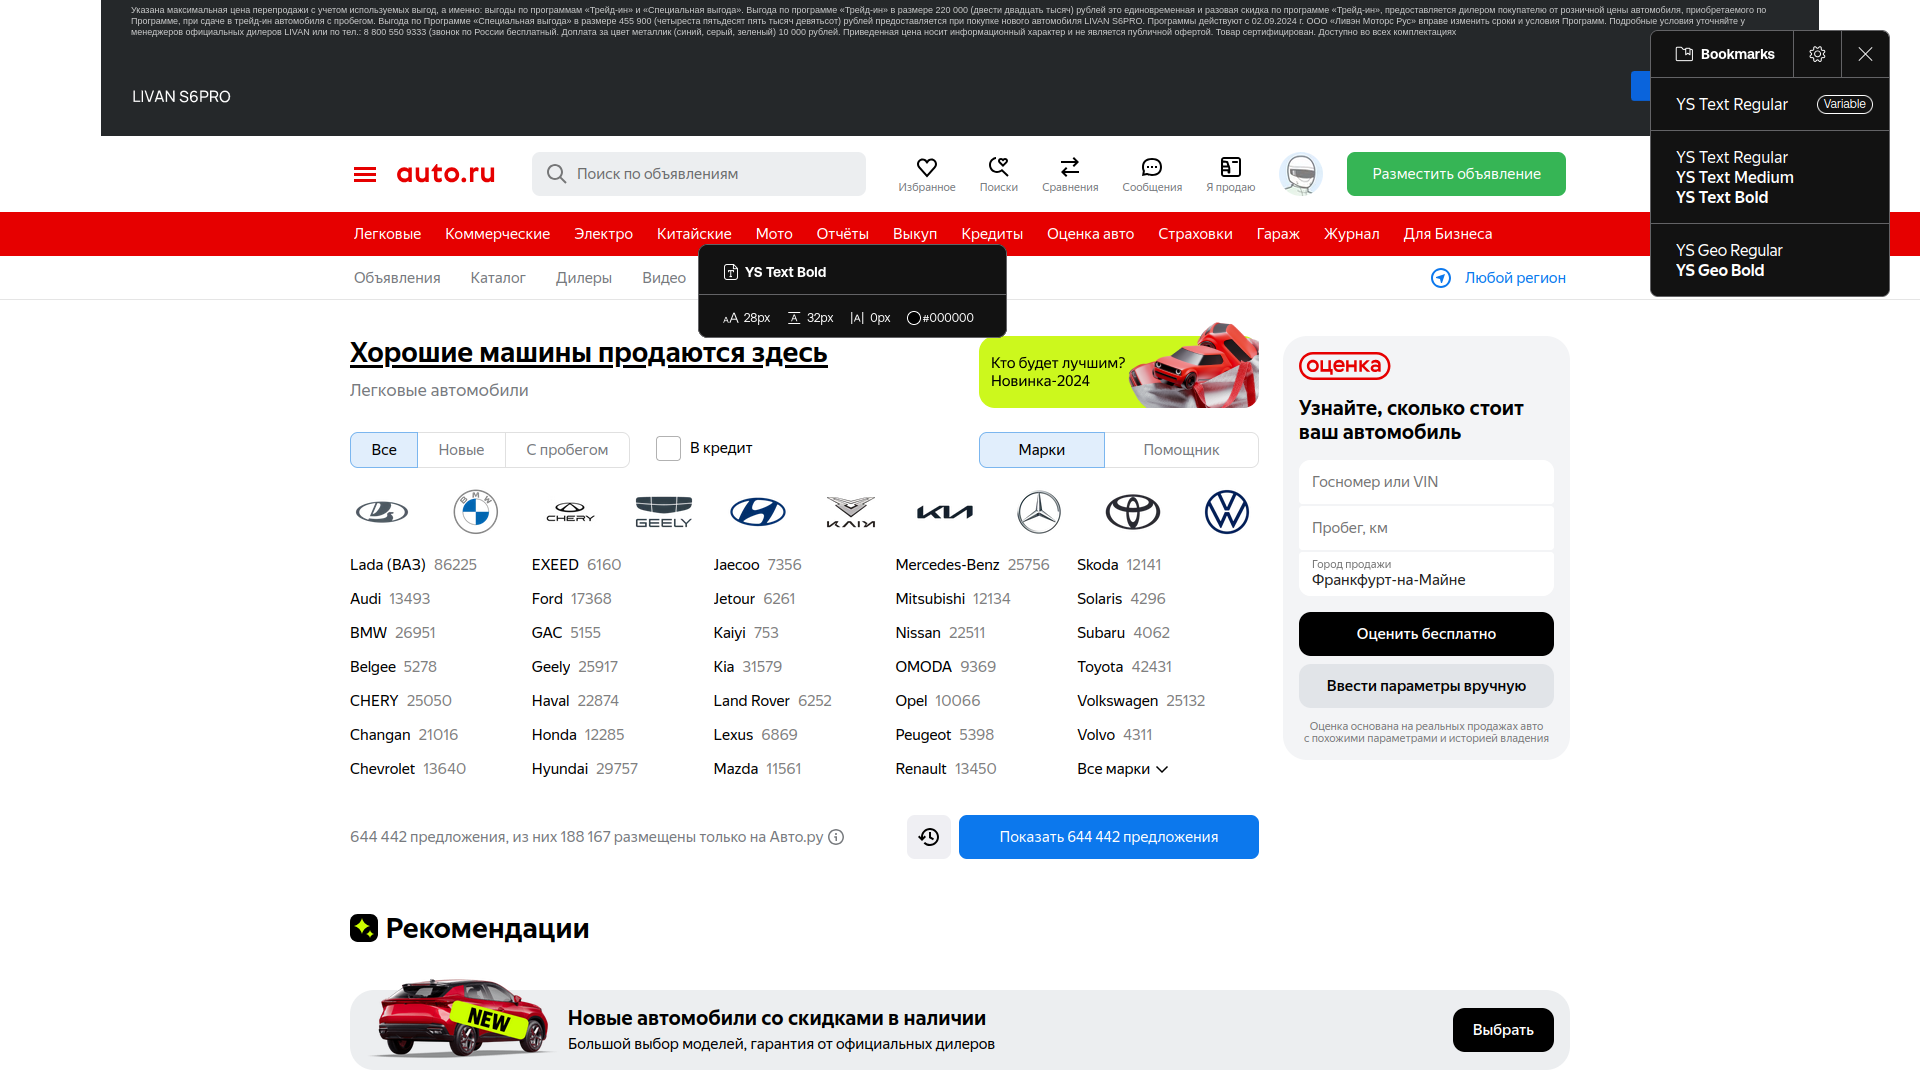
\includegraphics[width=\linewidth]{auto}}
    \captionof{figure}{auto.ru}
\end{minipage}
\bigskip

\noindent
\begin{minipage}{\linewidth}
    \fbox{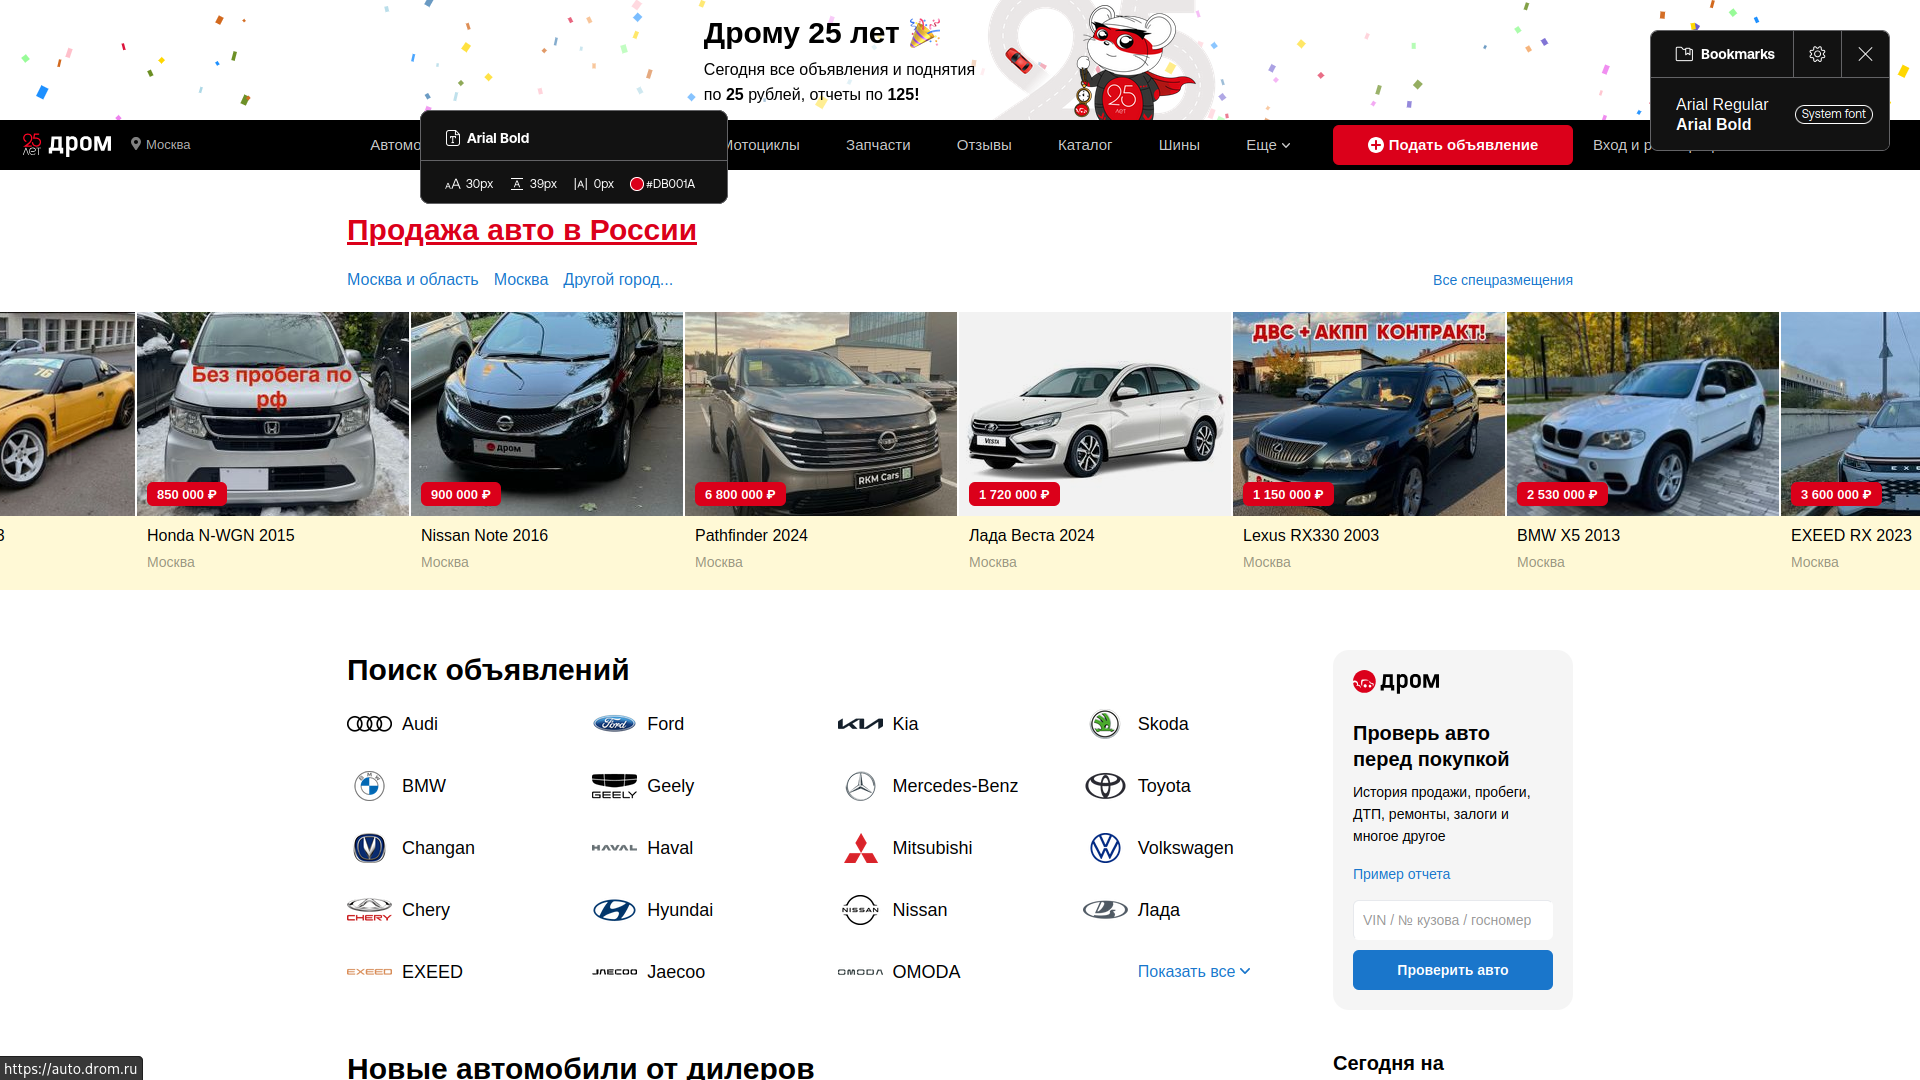
\includegraphics[width=\linewidth]{drom}}
    \captionof{figure}{drom.ru}
\end{minipage}
\bigskip

\noindent
\begin{minipage}{\linewidth}
    \fbox{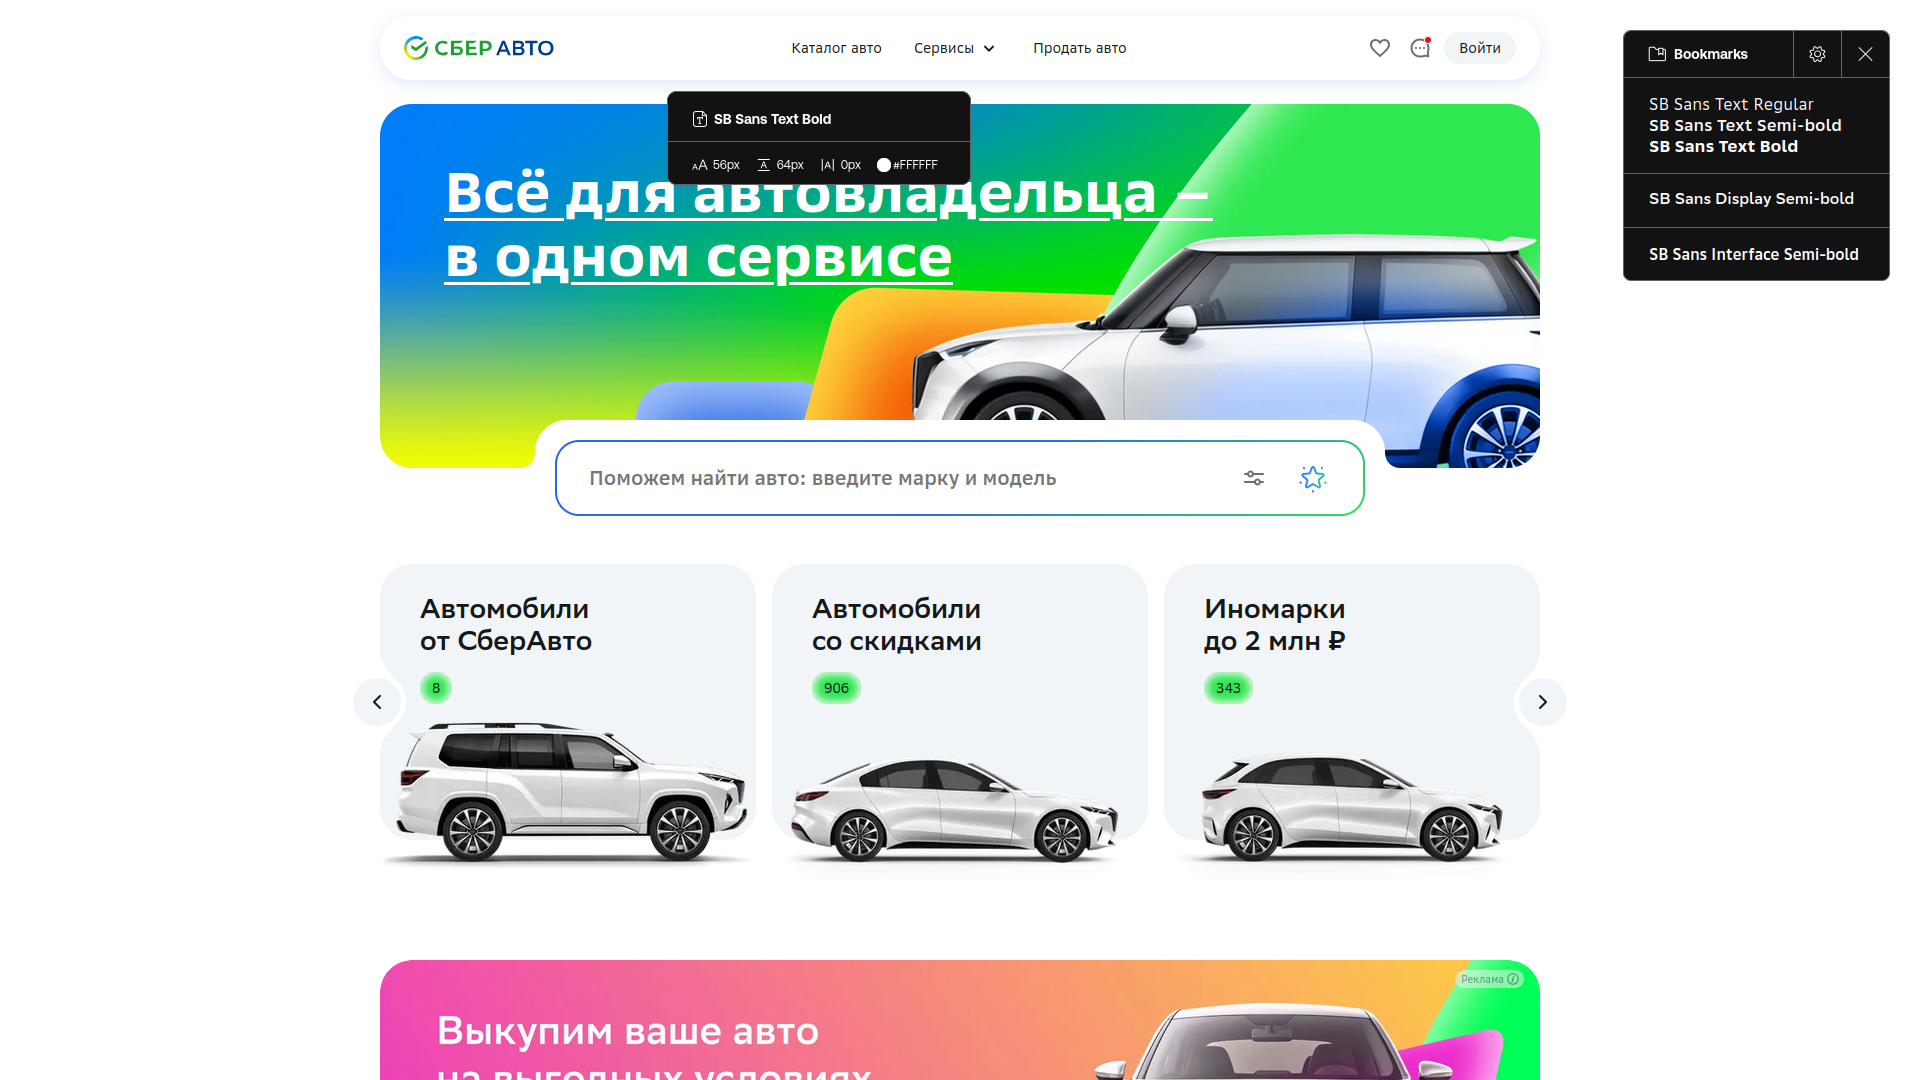
\includegraphics[width=\linewidth]{sberauto}}
    \captionof{figure}{sberauto.com}
\end{minipage}
\bigskip

\noindent
\begin{minipage}{\linewidth}
    \fbox{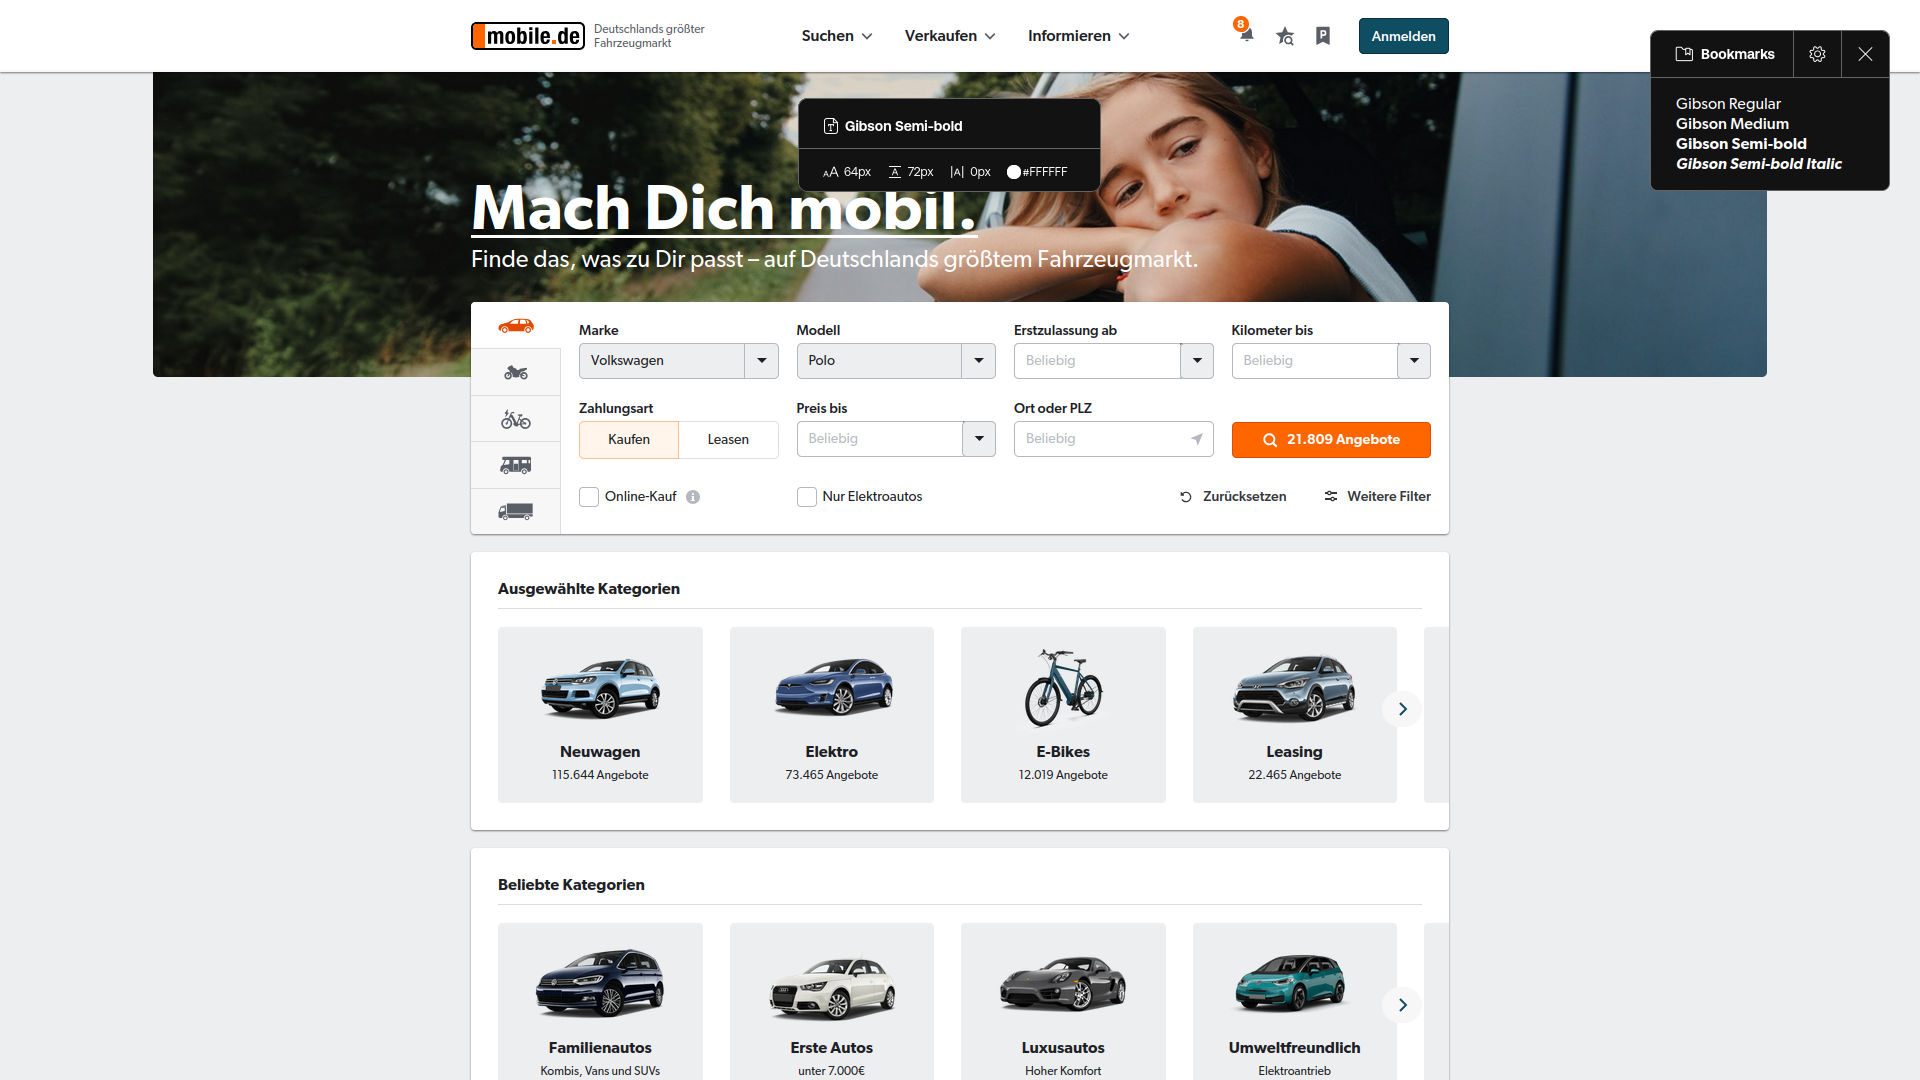
\includegraphics[width=\linewidth]{mobile}}
    \captionof{figure}{mobile.de}
\end{minipage}
\bigskip

\noindent
\begin{minipage}{\linewidth}
    \fbox{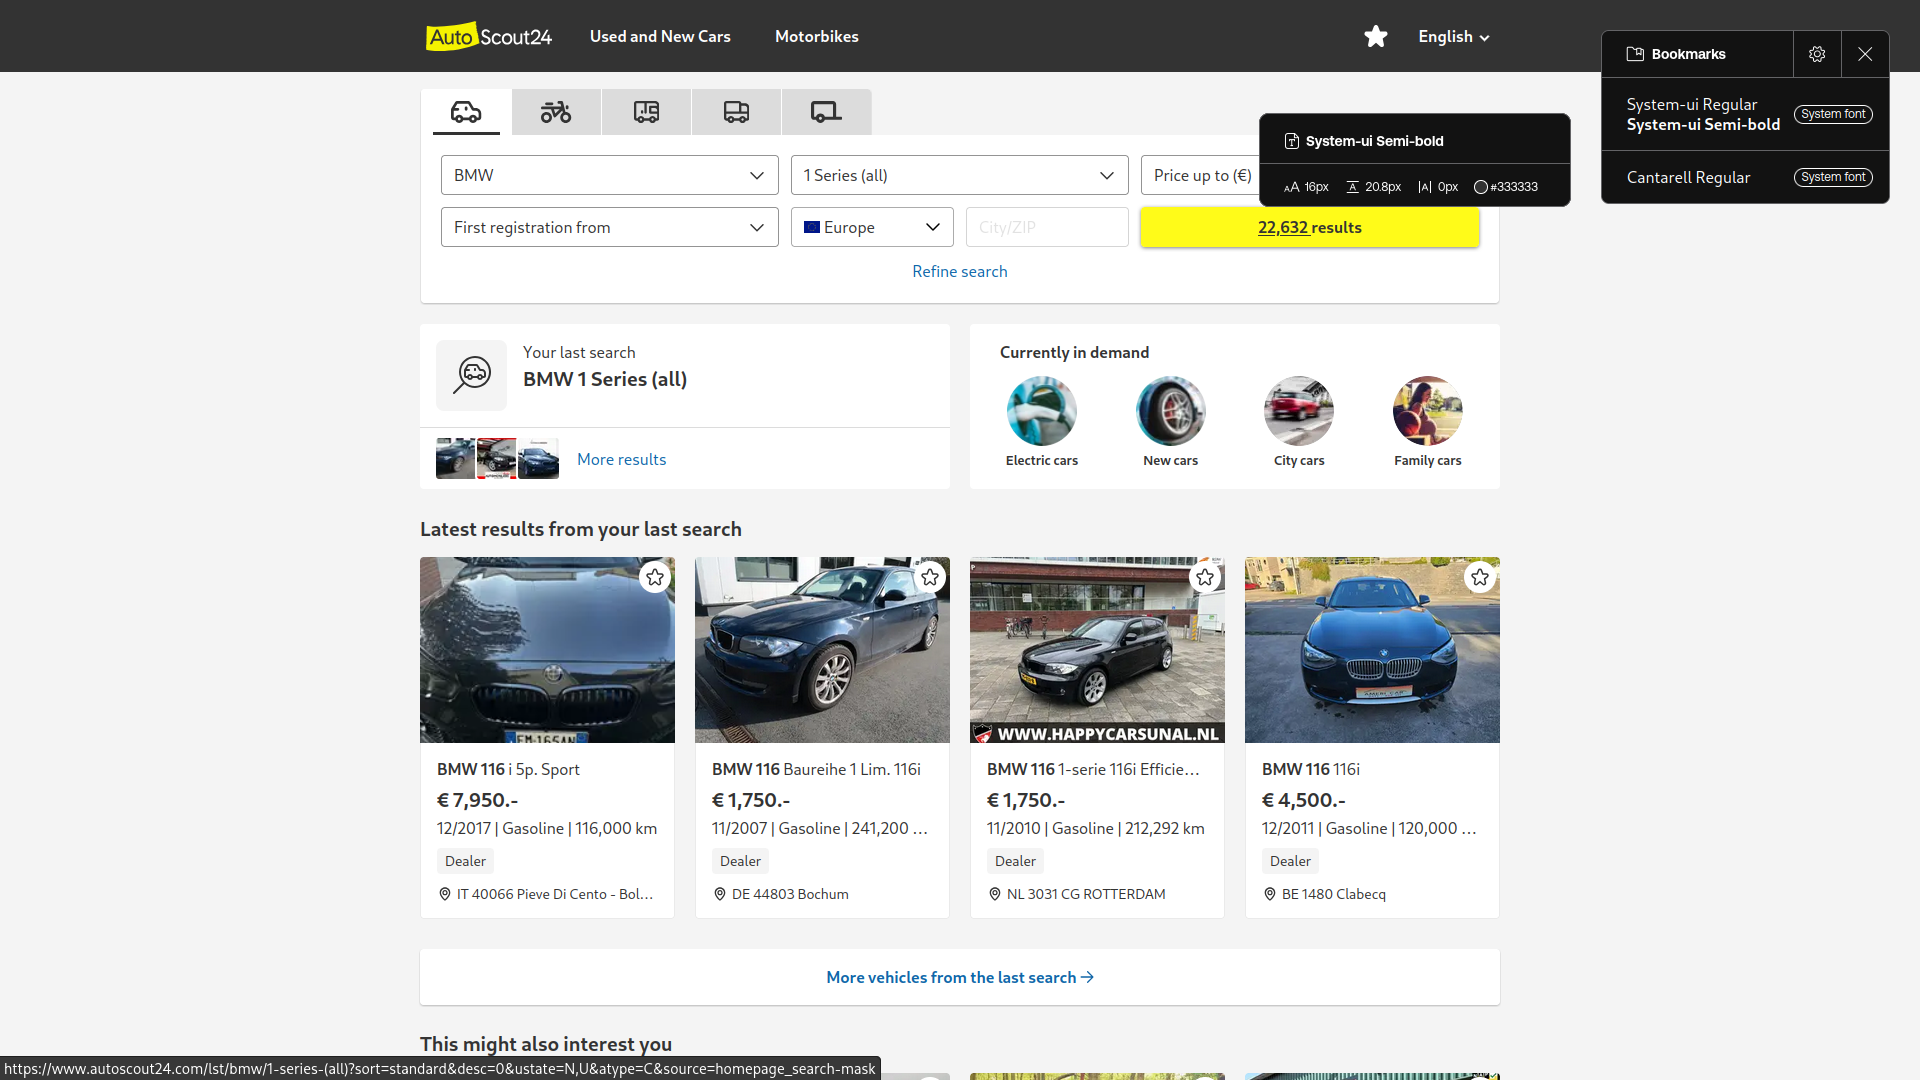
\includegraphics[width=\linewidth]{autoscout24}}
    \captionof{figure}{autoscout24.com}
\end{minipage}
\bigskip

\noindent
\begin{minipage}{\linewidth}
    \fbox{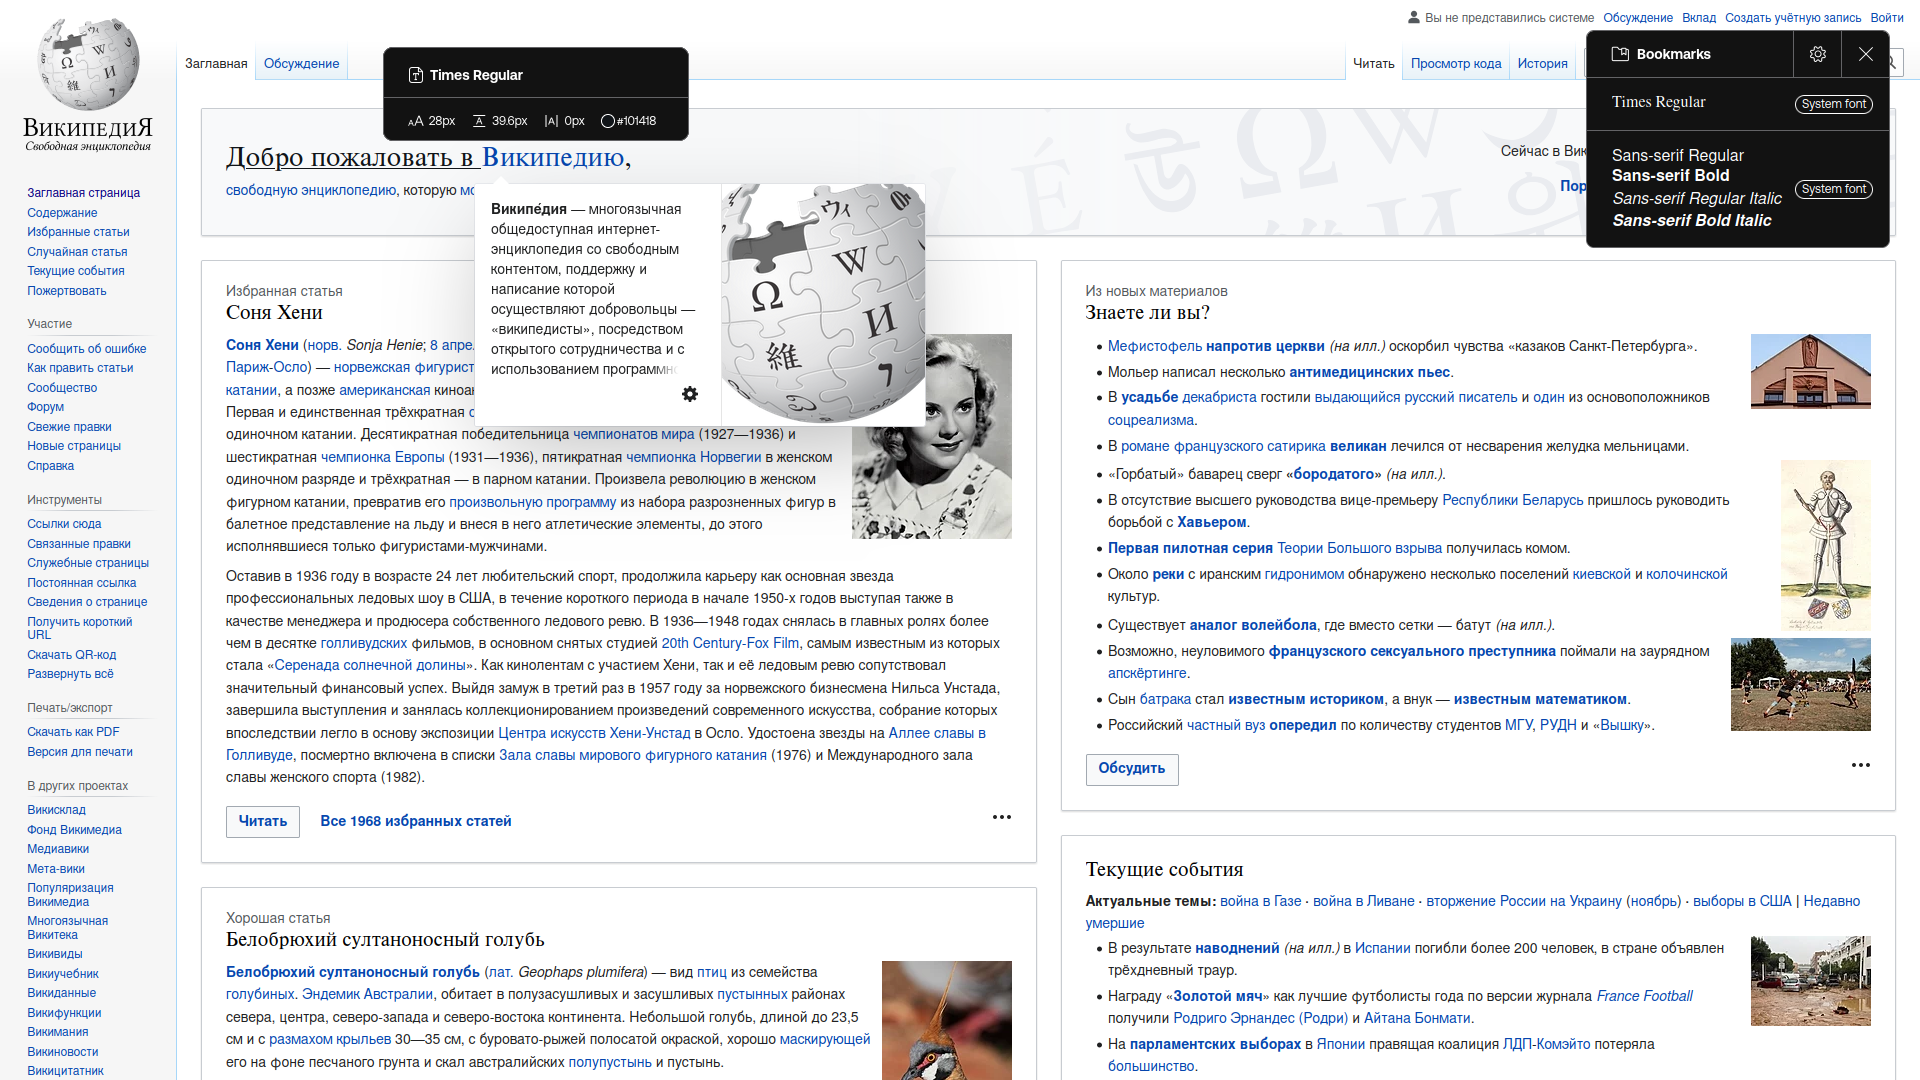
\includegraphics[width=\linewidth]{wikipedia}}
    \captionof{figure}{ru.wikipedia.org}
\end{minipage}
\bigskip

\noindent
\begin{minipage}{\linewidth}
    \fbox{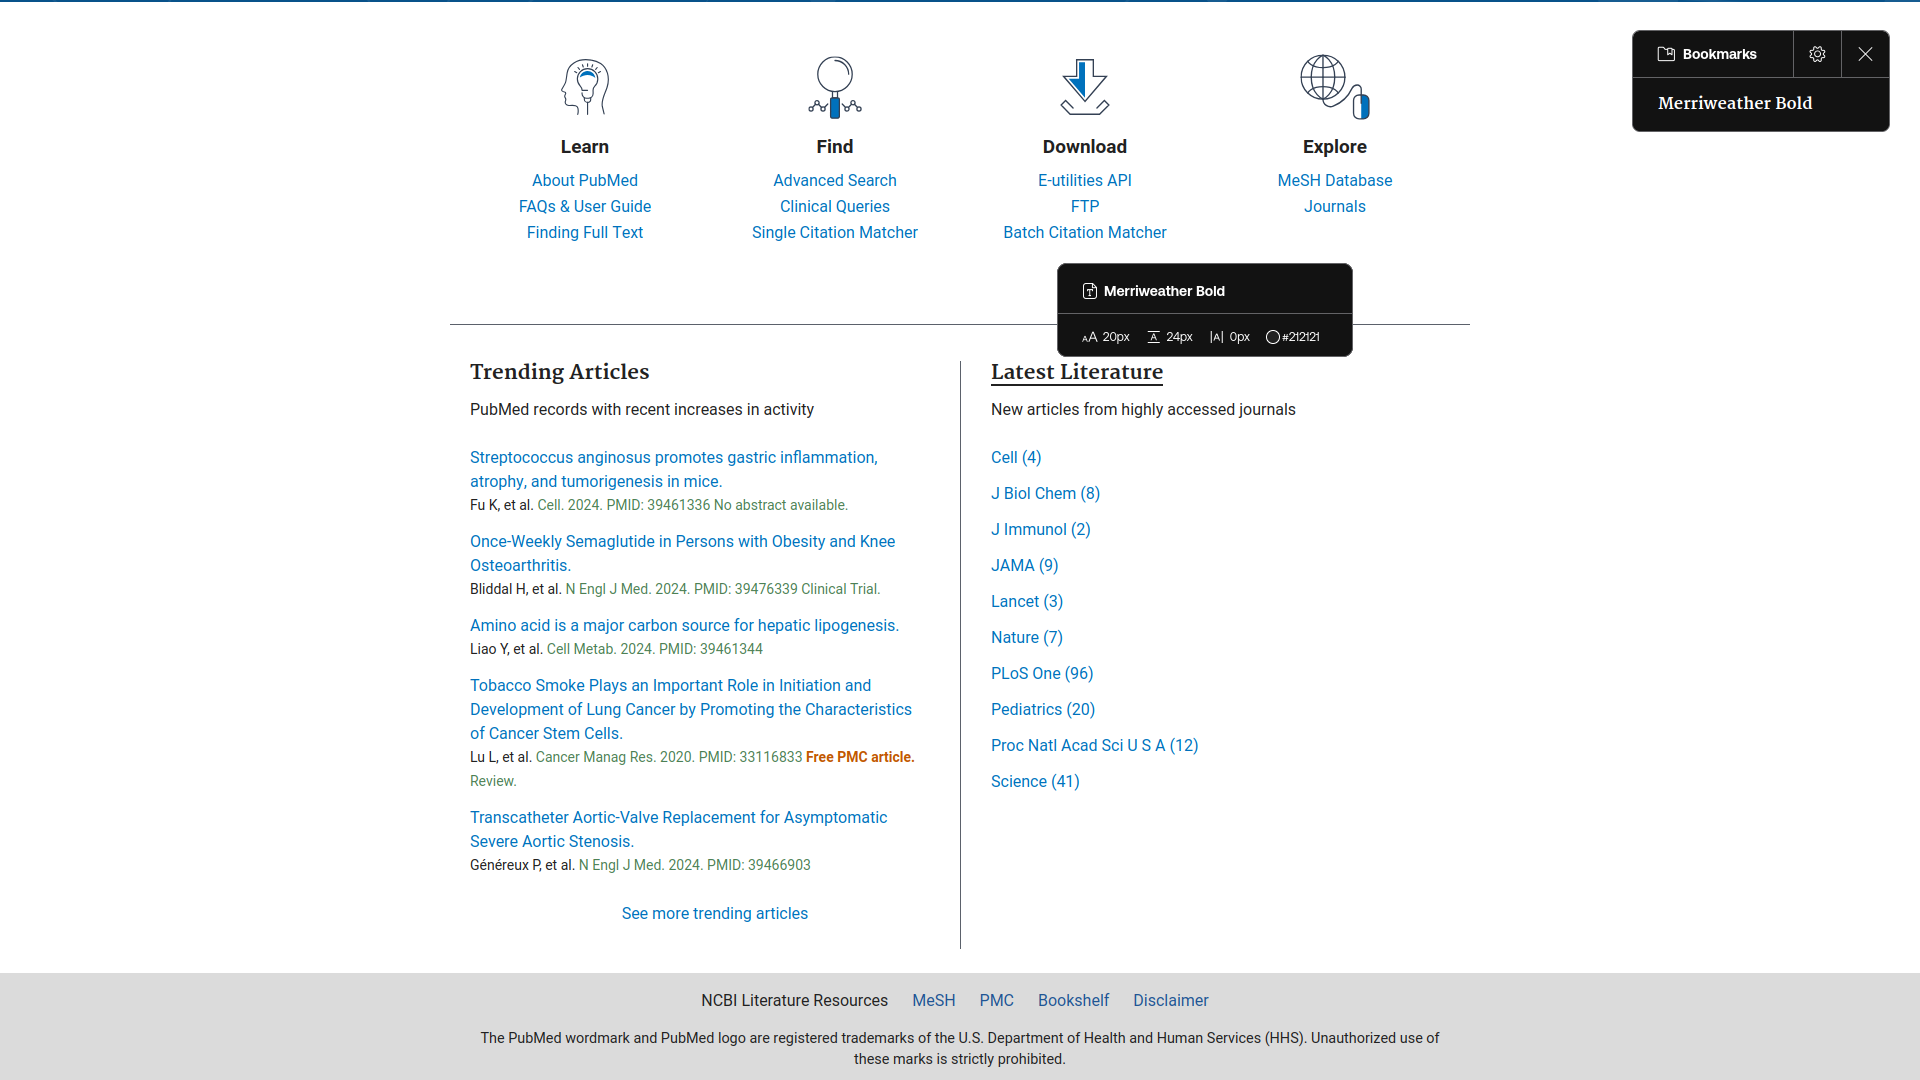
\includegraphics[width=\linewidth]{pubmed}}
    \captionof{figure}{pubmed.ncbi.nlm.nih.gov}
\end{minipage}
\bigskip

\noindent
\begin{minipage}{\linewidth}
    \fbox{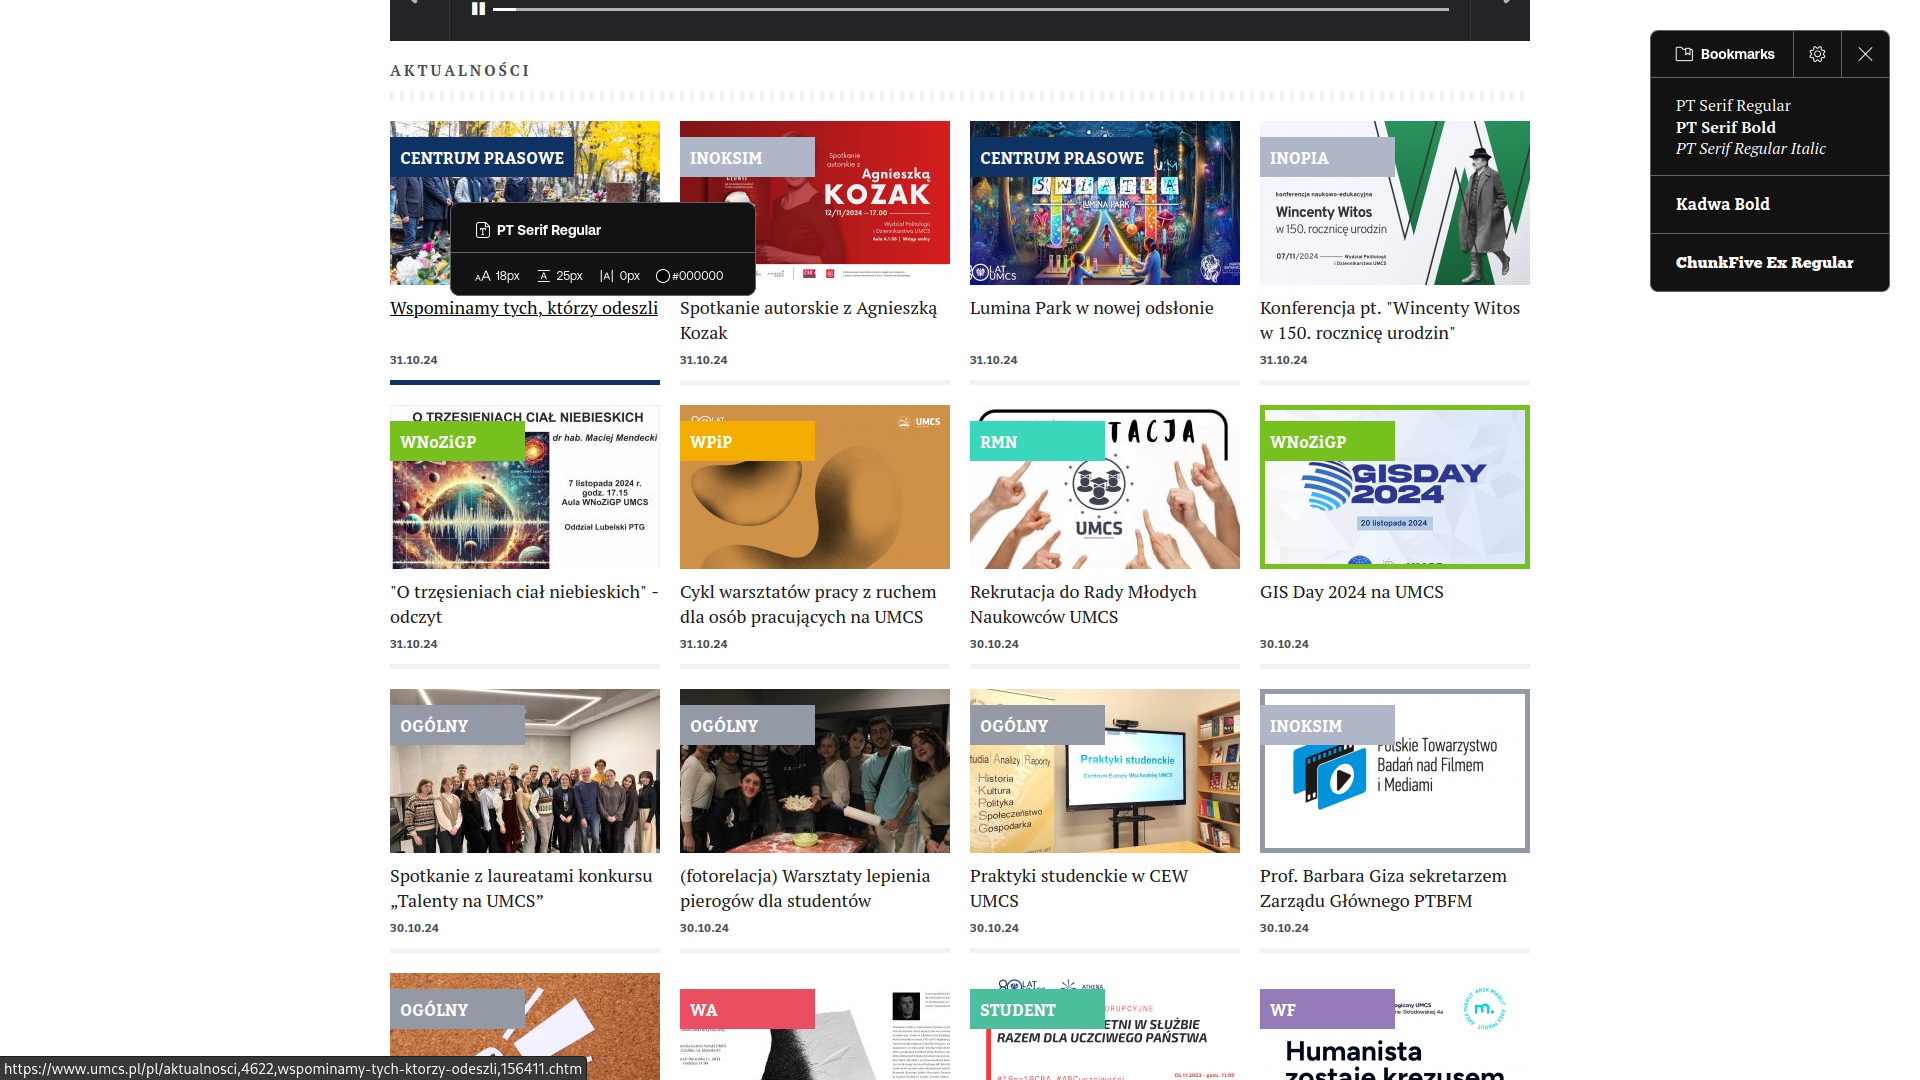
\includegraphics[width=\linewidth]{umcs}}
    \captionof{figure}{umcs.pl}
\end{minipage}
\bigskip

\noindent
\begin{minipage}{\linewidth}
    \fbox{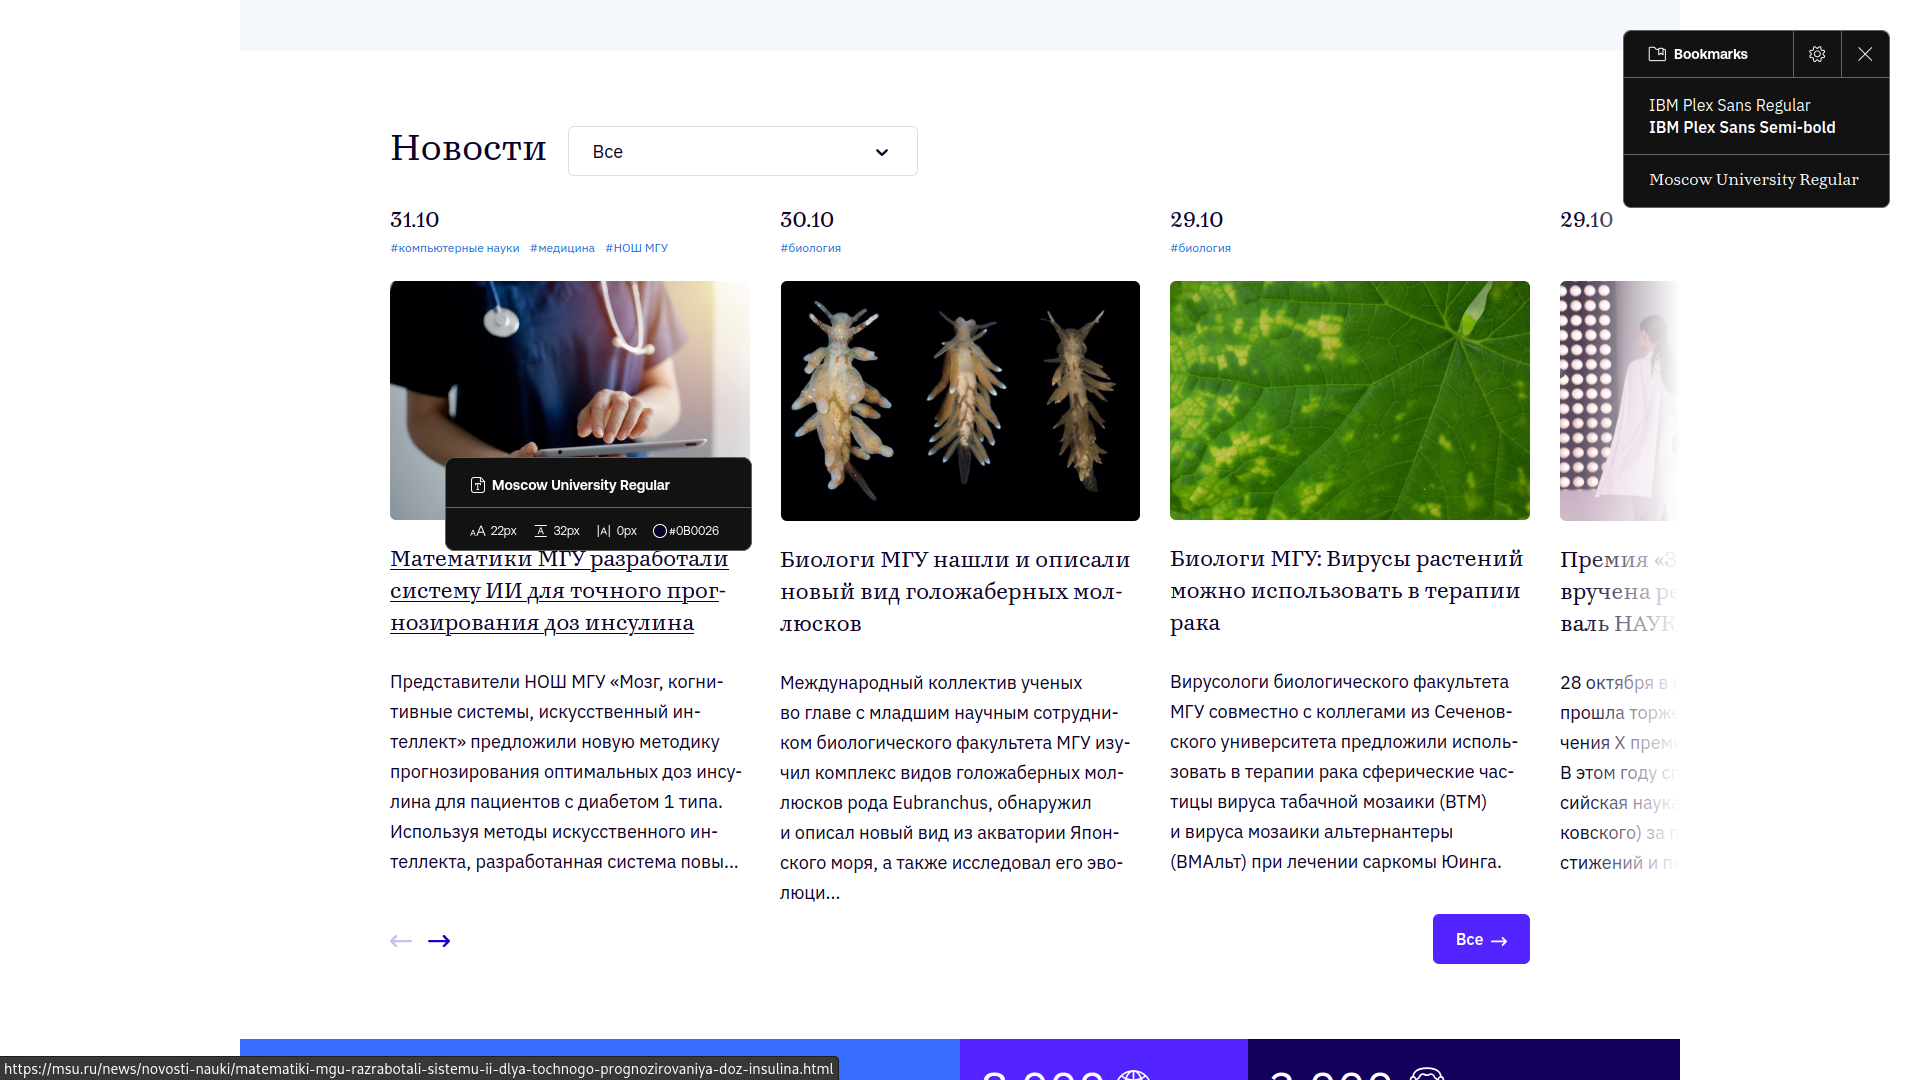
\includegraphics[width=\linewidth]{msu}}
    \captionof{figure}{msu.ru}
\end{minipage}
\bigskip

\noindent
\begin{minipage}{\linewidth}
    \fbox{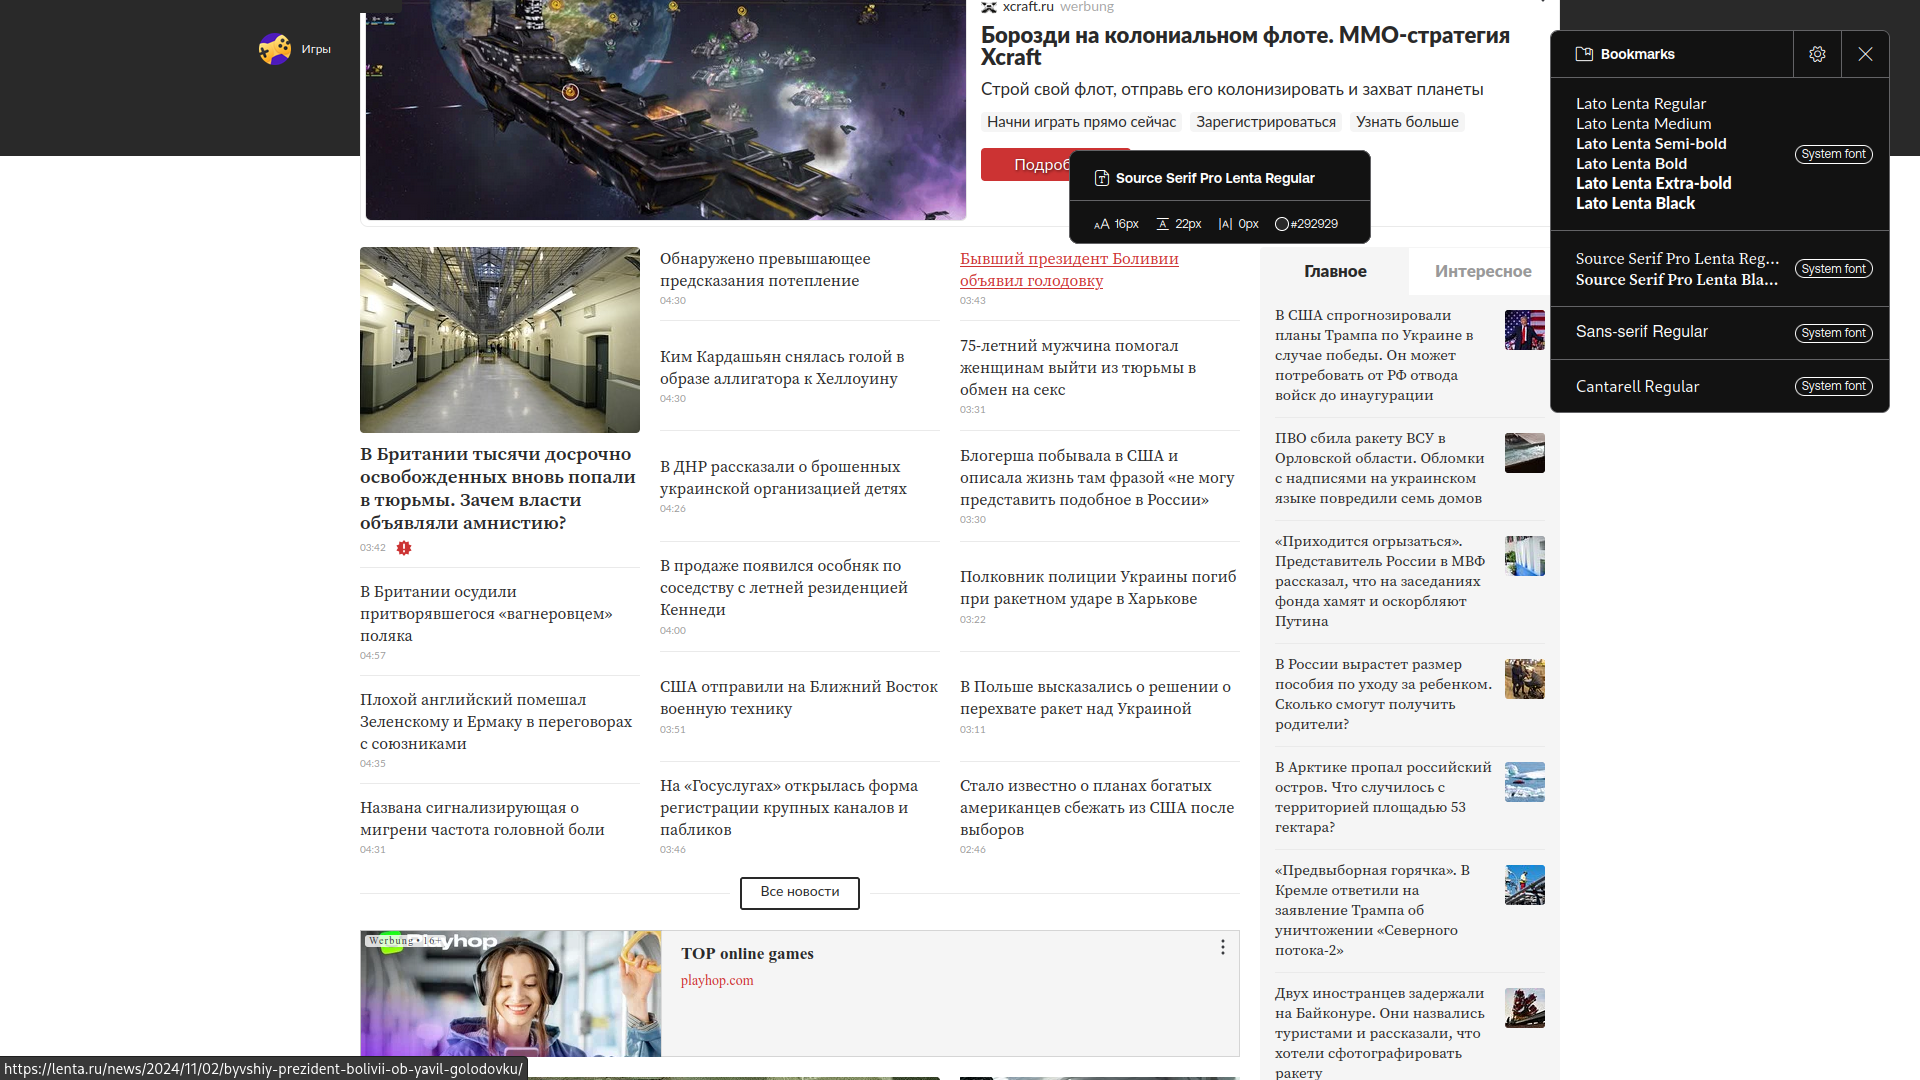
\includegraphics[width=\linewidth]{lenta}}
    \captionof{figure}{lenta.ru}
\end{minipage}
\bigskip

\noindent
\begin{minipage}{\linewidth}
    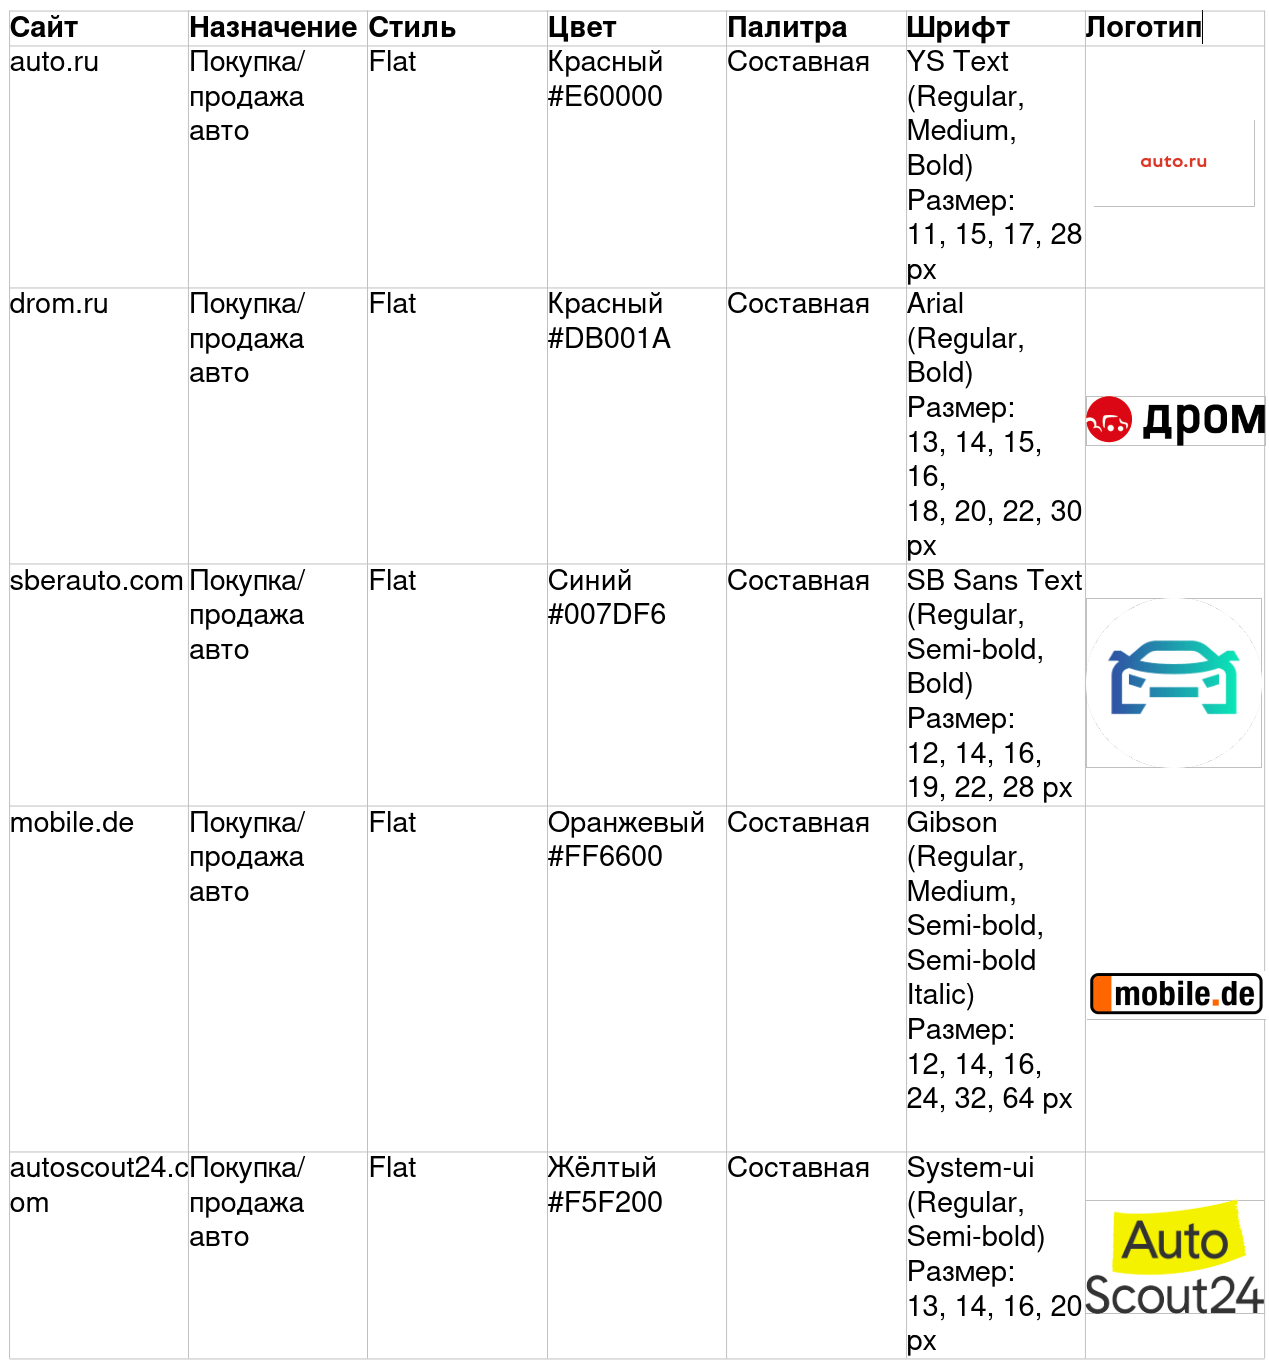
\includegraphics[width=\linewidth]{table}
\end{minipage}
\bigskip

\textbf{Выбор шрифтов для интерфейса}

По рекомендации сайта mixfont.com были выбраны шрифты Open Sans и Inter.
\bigskip

\noindent
\begin{minipage}{\linewidth}
    \fbox{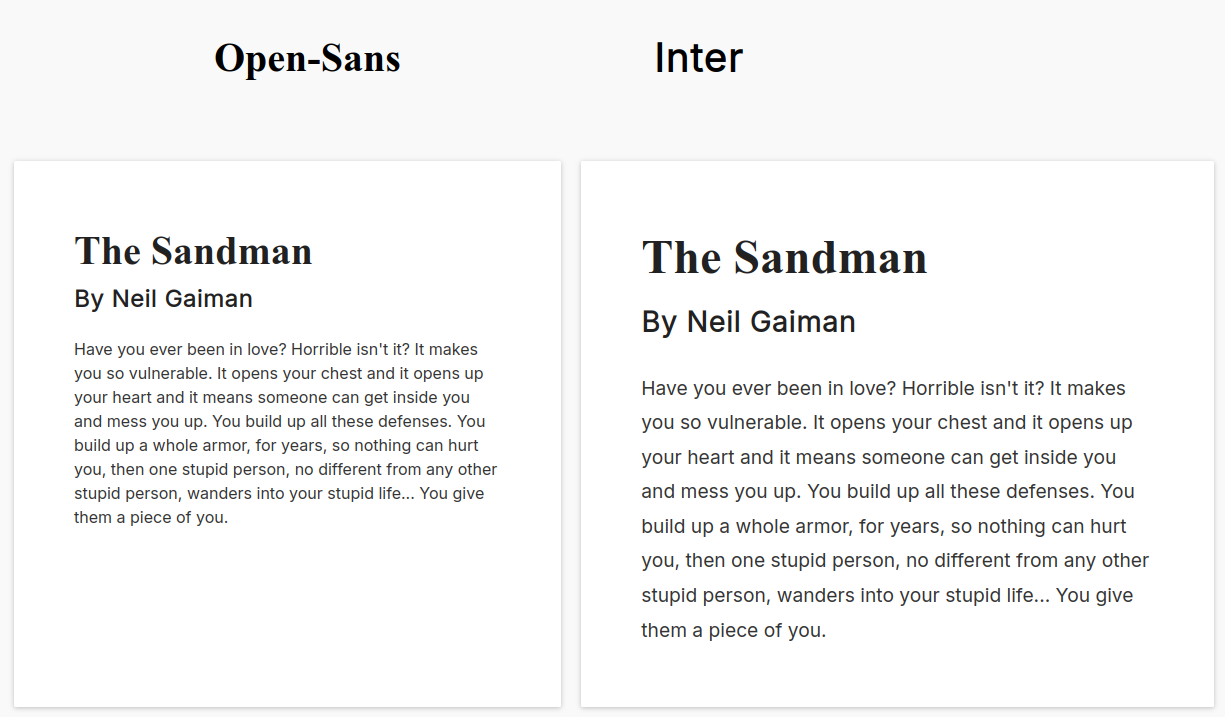
\includegraphics[width=\linewidth]{mixfont}}
    \captionof{figure}{mixfont.com Open Sans + Inter}
\end{minipage}
\bigskip

\noindent
\begin{minipage}{\linewidth}
    \fbox{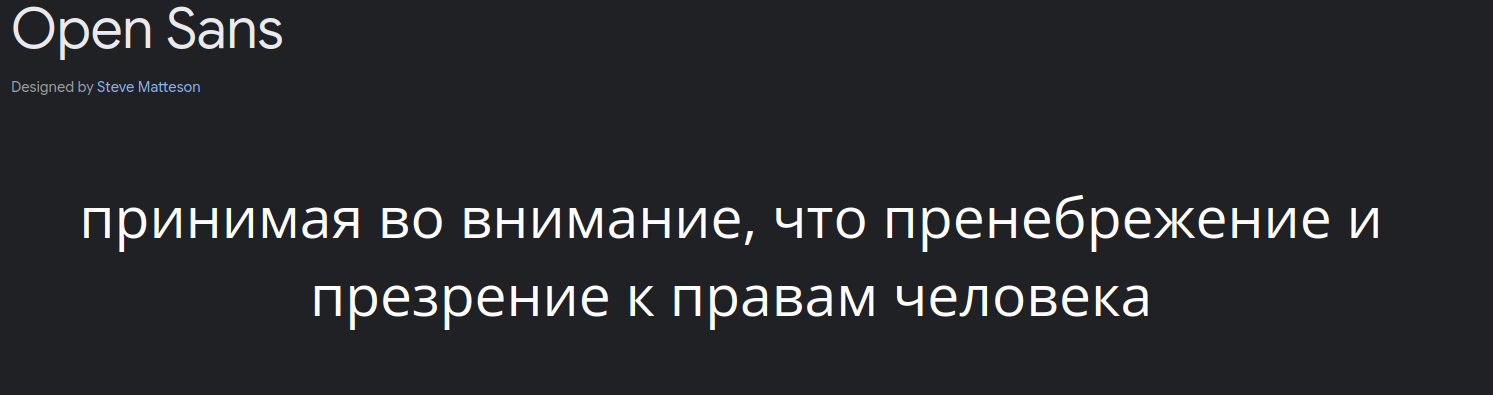
\includegraphics[width=\linewidth]{opensans}}
    \captionof{figure}{Open Sans кириллица}
\end{minipage}
\bigskip

\noindent
\begin{minipage}{\linewidth}
    \fbox{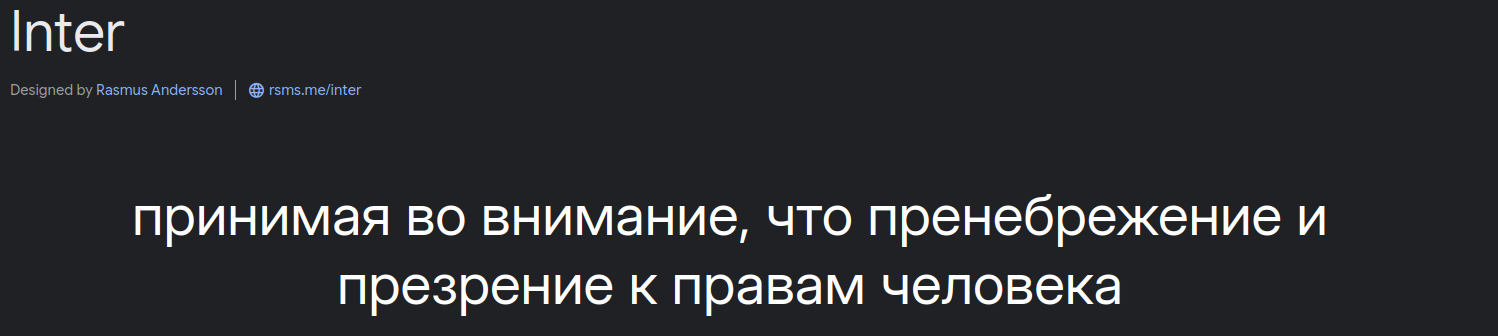
\includegraphics[width=\linewidth]{inter}}
    \captionof{figure}{Inter кириллица}
\end{minipage}
\bigskip

\noindent
\begin{minipage}{\linewidth}
    \fbox{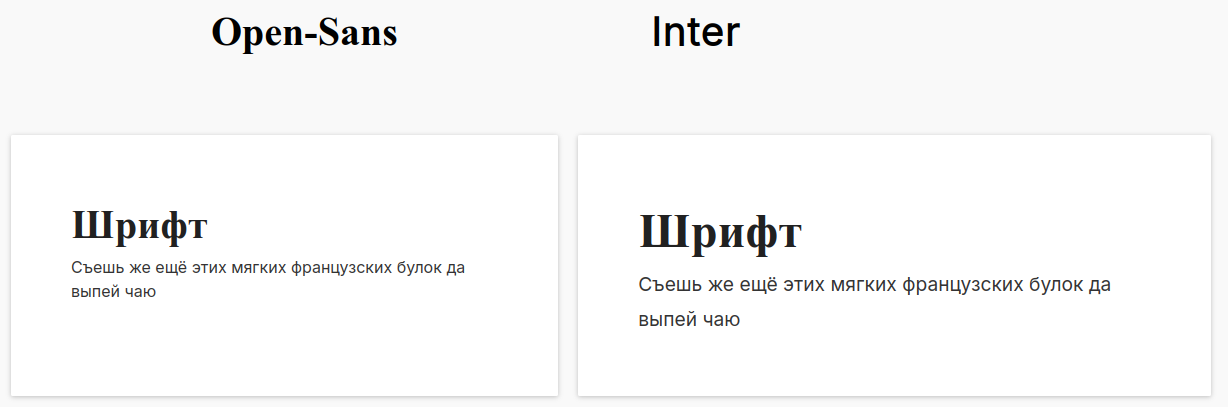
\includegraphics[width=\linewidth]{mix}}
\end{minipage}
\bigskip

\begin{enumerate}
    \item Заголовки

    Шрифт: Open Sans

        Основной заголовок (H1): 32–40 px, начертание: Bold.

        Подзаголовки (H2): 24–28 px, начертание: Semibold или Bold.

        Меньшие заголовки (H3): 20–24 px, начертание: Semibold.

    \item Текстовые блоки с основной информацией

    Шрифт: Inter

        Размер: 14–16 px, начертание: Regular

    \item Слова-акценты в тексте

    Шрифт: Inter или Open Sans - в зависимости от контекста

    Размер: соответствует основному тексту (14–16 px)

    Начертание: Italic, Semibold

    \item Рубрики

    Шрифт: Open Sans

    Размер: 18–20 px, начертание: Semibold

    \item Направляющие элементы

    Шрифт: Inter

        Кнопки и основные ссылки: 14–16 px, начертание: Bold или Semibold для акцента

        Метки и второстепенные элементы: 12–14 px, начертание: Regular или Semibold

\end{enumerate}
\bigskip

\textbf{Контрольные вопросы и ответы}

\begin{enumerate}
    \item Определение «Шрифта».

Шрифт – это набор графических символов (букв, цифр, знаков пунктуации и специальных символов), имеющих одинаковый стиль и размер. Шрифты бывают различных стилей (курсив, полужирный, подчеркнутый и т.д.) и начертаний (обычное, жирное, полужирное, курсивное и т.д.).

    \item Семейство, гарнитура, начертание шрифта

Семейство шрифтов: группа шрифтов, объединенных общим стилем.

Гарнитура: визуальная характеристика шрифта, объединяющая наборы символов с общими стилевыми признаками. Она может включать несколько начертаний и толщин.

Начертание: это вариант шрифта внутри гарнитуры, который может быть Regular, Bold, Italic и так далее.

\item Каковы критерии и принципы подбора типографики для текстового контента для веб?

Читаемость и удобочитаемость: шрифты должны легко читаться на экранах разных размеров.

Контраст и визуальная иерархия: крупные заголовки, средние подзаголовки и мелкий основной текст помогают структурировать текст и выделить важные моменты.

Универсальность: шрифты должны хорошо отображаться в разных браузерах и операционных системах. Лучше выбирать веб-оптимизированные шрифты.

Гибкость в настройке начертаний: для текстов разного уровня важности (заголовки, подзаголовки, текст) желательно использовать шрифт с доступом к различным начертаниям.

\item Каковы правила сочетания шрифтов, характеристики подбора пары.

    Контраст по стилю: сочетайте шрифты с разным стилем — например, Sans Serif для основного текста и Serif для заголовков. Это создаёт визуальную иерархию и улучшает восприятие.

    Контраст по толщине и насыщенности: используйте один шрифт с разными толщинами. Например, Inter для основного текста с Regular и Semibold для акцентов.

    Избегайте чрезмерной разнородности: обычно достаточно двух шрифтов для веб-сайта. Один для заголовков, второй для основного текста, чтобы не перегружать дизайн.

    Сходство по форме: шрифты должны гармонировать по общим чертам. Например, парой к Open Sans можно выбрать Merriweather, так как оба они отличаются современной читаемостью.

    \item Удобочитаемость шрифта

Удобочитаемость шрифта зависит от нескольких факторов, включая размер, начертание, интерлиньяж (расстояние между строками), контрастность и цвет фона. Убедитесь, что ваш выбранный шрифт обеспечивает хорошую читаемость на всех устройствах и разрешениях экрана.

    \item Проверка коэффициента контрастности. Регламентирующие документы.

Для проверки коэффициента контрастности между текстом и фоном можно использовать онлайн-инструменты, такие как WebAIM's Color Contrast Checker или Contrast Checker от W3C. Регламентирующие документы, такие как Web Content Accessibility Guidelines (WCAG), также содержат рекомендации по минимальным требованиям к контрастности для обеспечения доступности контента для всех пользователей, включая людей с ограниченными возможностями.
\end{enumerate}

\end{document}
